%=============================================================================
%  Standalone wrapper -- fig_phases
%
%      pdflatex main.tex
%
%  The paper places this figure in a \begin{figure*} of
%  \documentclass[prx,amsmath,amssymb,twocolumn,superscriptaddress]{revtex4-2},
%  where \linewidth is 510.0pt. The figure is written in terms of \linewidth, so
%  that length has to be reproduced here or the output is scaled differently.
%
%  The standalone class's `varwidth' option does NOT do this: with the `tikz'
%  option the class crops to the picture and leaves \linewidth at its own
%  default of 345.0pt. The lengths are therefore set explicitly below.
%=============================================================================
\documentclass[border=0pt,tikz,10pt]{standalone}
% NOT lmodern: revtex4-2 prx typesets figures in Computer Modern (cmr).
\usepackage{graphicx}
\usepackage{csvsimple}
\usepackage{tikzscale}
\usepackage{amsmath, esint}
\usepackage{amsfonts}
\usepackage{amssymb}
\usepackage{xcolor}
\setcounter{secnumdepth}{3}
%\usepackage[francais]{babel}
\usepackage[english]{babel}
% \usepackage{indentfirst}
\selectlanguage{english}
%\usepackage[utf8]{inputenc}
%\usepackage[T1]{fontenc}
%\usepackage{float}
\usepackage[colorlinks,bookmarks=false,linkcolor=blue,urlcolor=blue, citecolor=black]{hyperref}
\usepackage{placeins}
\usepackage{ulem}
\usepackage[squaren, cdot]{SIunits}
\usepackage{sistyle}
\usepackage{epstopdf}
%\usepackage{color}
\usepackage{pgf, tikz}
\usetikzlibrary{arrows,shapes,positioning}
\usetikzlibrary{datavisualization}
\usetikzlibrary{datavisualization.formats.functions}
\usetikzlibrary[
pgfplots.groupplots,
decorations,
decorations.pathmorphing,
decorations.pathreplacing,
decorations.text,
decorations.markings,
backgrounds,
chains,
calc,
automata,
arrows.meta,
intersections
]
\usepackage{scalefnt}
\usepackage{caption}
\usepackage{multirow}
\usepackage{wrapfig}
\usepackage{chemfig}
\usepackage{chemarr}
\usepackage{listings}
\usepackage{inconsolata}
\usepackage{color} 
\usepackage{pgfplots}
\usepgfplotslibrary{colormaps}
\usepackage{pgfplotstable}
\usepackage{svg}
\pgfplotsset{compat=newest}
\pgfplotstableset{col sep=comma}
\usepackage{cancel}
\usepackage{dirtytalk}
\usepackage{float}
\usepackage[export]{adjustbox}
\usepackage{pdfpages}

\definecolor{Gray}{rgb}{0.5, 0.5, 0.5}
\definecolor{Blue}{rgb}{0.0, 0.0, 1.0}
\definecolor{Olive}{rgb}{0.5, 0.5, 0.0}
\definecolor{Maroon}{rgb}{0.5, 0.0, 0.0}
\definecolor{applegreen}{rgb}{0.55, 0.71, 0.0}
\definecolor{ao}{rgb}{0.0, 0.5, 0.0}
\definecolor{bleudefrance}{rgb}{0.19, 0.55, 0.91}
\definecolor{actincolor}{HTML}{ffc311}
\definecolor{nuccolor}{HTML}{0600ff}
\definecolor{myosincolor}{HTML}{26a22b}
\definecolor{cyan}{rgb}{0.0, 1.0, 1.0}
\definecolor{RdPu1}{HTML}{feebe2}
\definecolor{RdPu2}{HTML}{f768a1}
\definecolor{RdPu3}{HTML}{7a0177}

% The paper's preamble inputs abrv.tex; the figures use its shorthands
% (\zr, \Dmu, ...). Without it they silently vanish from the output.
\def\a{\alpha}
\def\b{\beta}
\def\g{\gamma}
\def\d{\delta}
\def \ga {g_\a}
\def \wab {\omega_{\alpha\beta}}
\def \wag {\omega_{\alpha\gamma}}
\def \vab {v_{\alpha\beta}}
\def \vga {v_{\g\a}}
\def \vgb {v_{\g\beta}}
\def \vbg {v_{\b\g}}
\def \vgd {v_{\g\d}}
\def \vag {v_{\alpha\g}}
\def \vad {v_{\alpha\d}}
\def \vbd {v_{\b\d}}
\def \vgg {v_{\g\g}}
\def \vdd {v_{\d\d}}
\def \vbb {v_{\b\b}}
\def \vzz {v_{zz}}
\def \vxx {v_{xx}}
\def \vxz {v_{xz}}
\def \dab {\delta_{\alpha\beta}}
\def \va {v_\alpha}
\def \vb {v_\beta}
\def \vx {v_x}
\def \vy {v_y}
\def \vz {v_z}
\def \pt {\partial_t}
\def \pa {\partial_\alpha}
\def \pb {\partial_\beta}
\def \pg {\partial_\gamma}
\def \pe {\partial_\varepsilon}
\def\pd{{\partial_\delta}}
\def \pn {\partial_n}
\def \px {\partial_x}
\def \pz {\partial_z}
\def \pzz {\partial_{zz}}
\def \Pa {{P_\alpha}}
\def \Px {{P_x}}
\def \Py {{P_y}}
\def \Pap {{P'_\alpha}}
\def \Pb {{P_\beta}}
\def \Pg {{P_\gamma}}
\def \Pd {{P_\delta}}
\def \Pn {{P_\nu}}
\def \Px {{P_x}}
\def \Pz {{P_z}}
\def \Qab {{Q_\ab}}
\def \Qba {{Q_{\beta\alpha}}}
\def \Qabp {{Q'_\ab}}
\def \Qag {Q_{\a\gamma}}
\def \Qbg {Q_{\beta\gamma}}
\def \Qgb {Q_{\gamma\beta}}
\def \Qgd {Q_{\gamma\delta}}
\def \Qdd {Q_{\d\d}}
\def \Qgg {Q_{\g\g}}
\def \Qbd {Q_{\b\delta}}
\def \Qdg {Q_{\delta\gamma}}
\def \Qad {Q_{\alpha\delta}}
\def \Qam {Q_{\alpha\mu}}
\def \Qma {Q_{\mu\a}}
\def \Qbm {Q_{\b\mu}}
\def \Qmb {Q_{\mu\b}}
\def \Qxx {Q_{xx}}
\def \Qxz {Q_{xz}}
\def \Qzz {Q_{zz}}
\def \ga {{g_\alpha}}
\def\ha{{h_\alpha}}
\def\hb{{h_\beta}}
\def\hd{{h_\d}}
\def\hg{{h_\g}}
\def\hx{{h_x}}
\def\hz{{h_z}}
\def \Hab{{H_\ab}}
\def \Hbg{{H_{\beta\gamma}}}
\def \Hgb{{H_{\g\b}}}
\def \Hbb{{H_{\b\b}}}
\def \Hgg{{H_{\g\gamma}}}
\def \Hag{{H_{\a\g}}}
\def \Hga{{H_{\g\a}}}
\def \Had{{H_{\a\d}}}
\def \Hdg{{H_{\d\gamma}}}
\def \Hbd{{H_{\b\d}}}
\def \Hgd{{H_{\gamma\d}}}
\def \Ham {H_{\alpha\mu}}
\def \Hma {H_{\mu\a}}
\def \Hbm {H_{\b\mu}}
\def \Hmb {H_{\mu\b}}
\def \Hxx {H_{xx}}
\def \Hxz {H_{xz}}
\def \Hzz {H_{zz}}
\def \sab {\sigma_\ab}
\def \sdab {\sigma_\ab^\text{d}}
\def \stab {\sigma_\ab^\text{tot}}
\def \staab {\sigma_\ab^\text{tot,a}}
\def \seab {\sigma_\ab^\text{e}}
\def \seaab {\sigma_\ab^\text{e,a}}
\def \saab {\sigma_\ab^\text{a}}
\def \sege {\sigma_{\g\varepsilon}^\text{e}}
\def\pPa {\partial_\Pa}
\def\pQab {\partial_\Qab}
\def\dr{\dd^3\v r}
\def\ra{{r_\alpha}}
\def\rd{{r_\delta}}
\def\rg{r_\gamma}
\def\vr{{\v r}}
\def\Mabe{{M_{\a\b\varepsilon}}}
\def\Mabg{{M_{\a\b\g}}}
\def\Dt{{\rm D}_t}
\def\Dmu{\Delta\mu}
\def \ar {a_\rho}
\def \ap {a_P}
\def \kp {k_P}
\def \aq {a_Q}
\def \kq {k_Q}
\def \zp {\zeta_P}
\def \zr {\zeta_\rho}
\def \zq {\zeta_Q}

\def \sab {\sigma_\ab}
\def \vntab {\vab^{tl}}
\def \vdiab {\vab^{di}}
\def \sntab {\sab^{tl}}
\def \sdiab {\sab^{di}}
\input{some_command}

\setlength{\parindent}{0pt}


% --- reproduce the paper's text block for this figure --------------------
\setlength{\textwidth}{510.0pt}
\setlength{\columnwidth}{510.0pt}
\setlength{\linewidth}{510.0pt}
\setlength{\hsize}{510.0pt}

\begin{document}%
% revtex4-2 sets 9pt/10.5pt inside figure environments; match it so text
% nodes and axis labels come out at the paper's size.
\fontsize{9}{10.5}\selectfont%
\begin{tikzpicture}
\def\lx{0.95}
\def\offx{0.05*\linewidth}
\def\cx{0.5*\linewidth-\offx}
\node[inner sep=0pt, anchor=south west, align=left] (heat) at (-\offx,0) {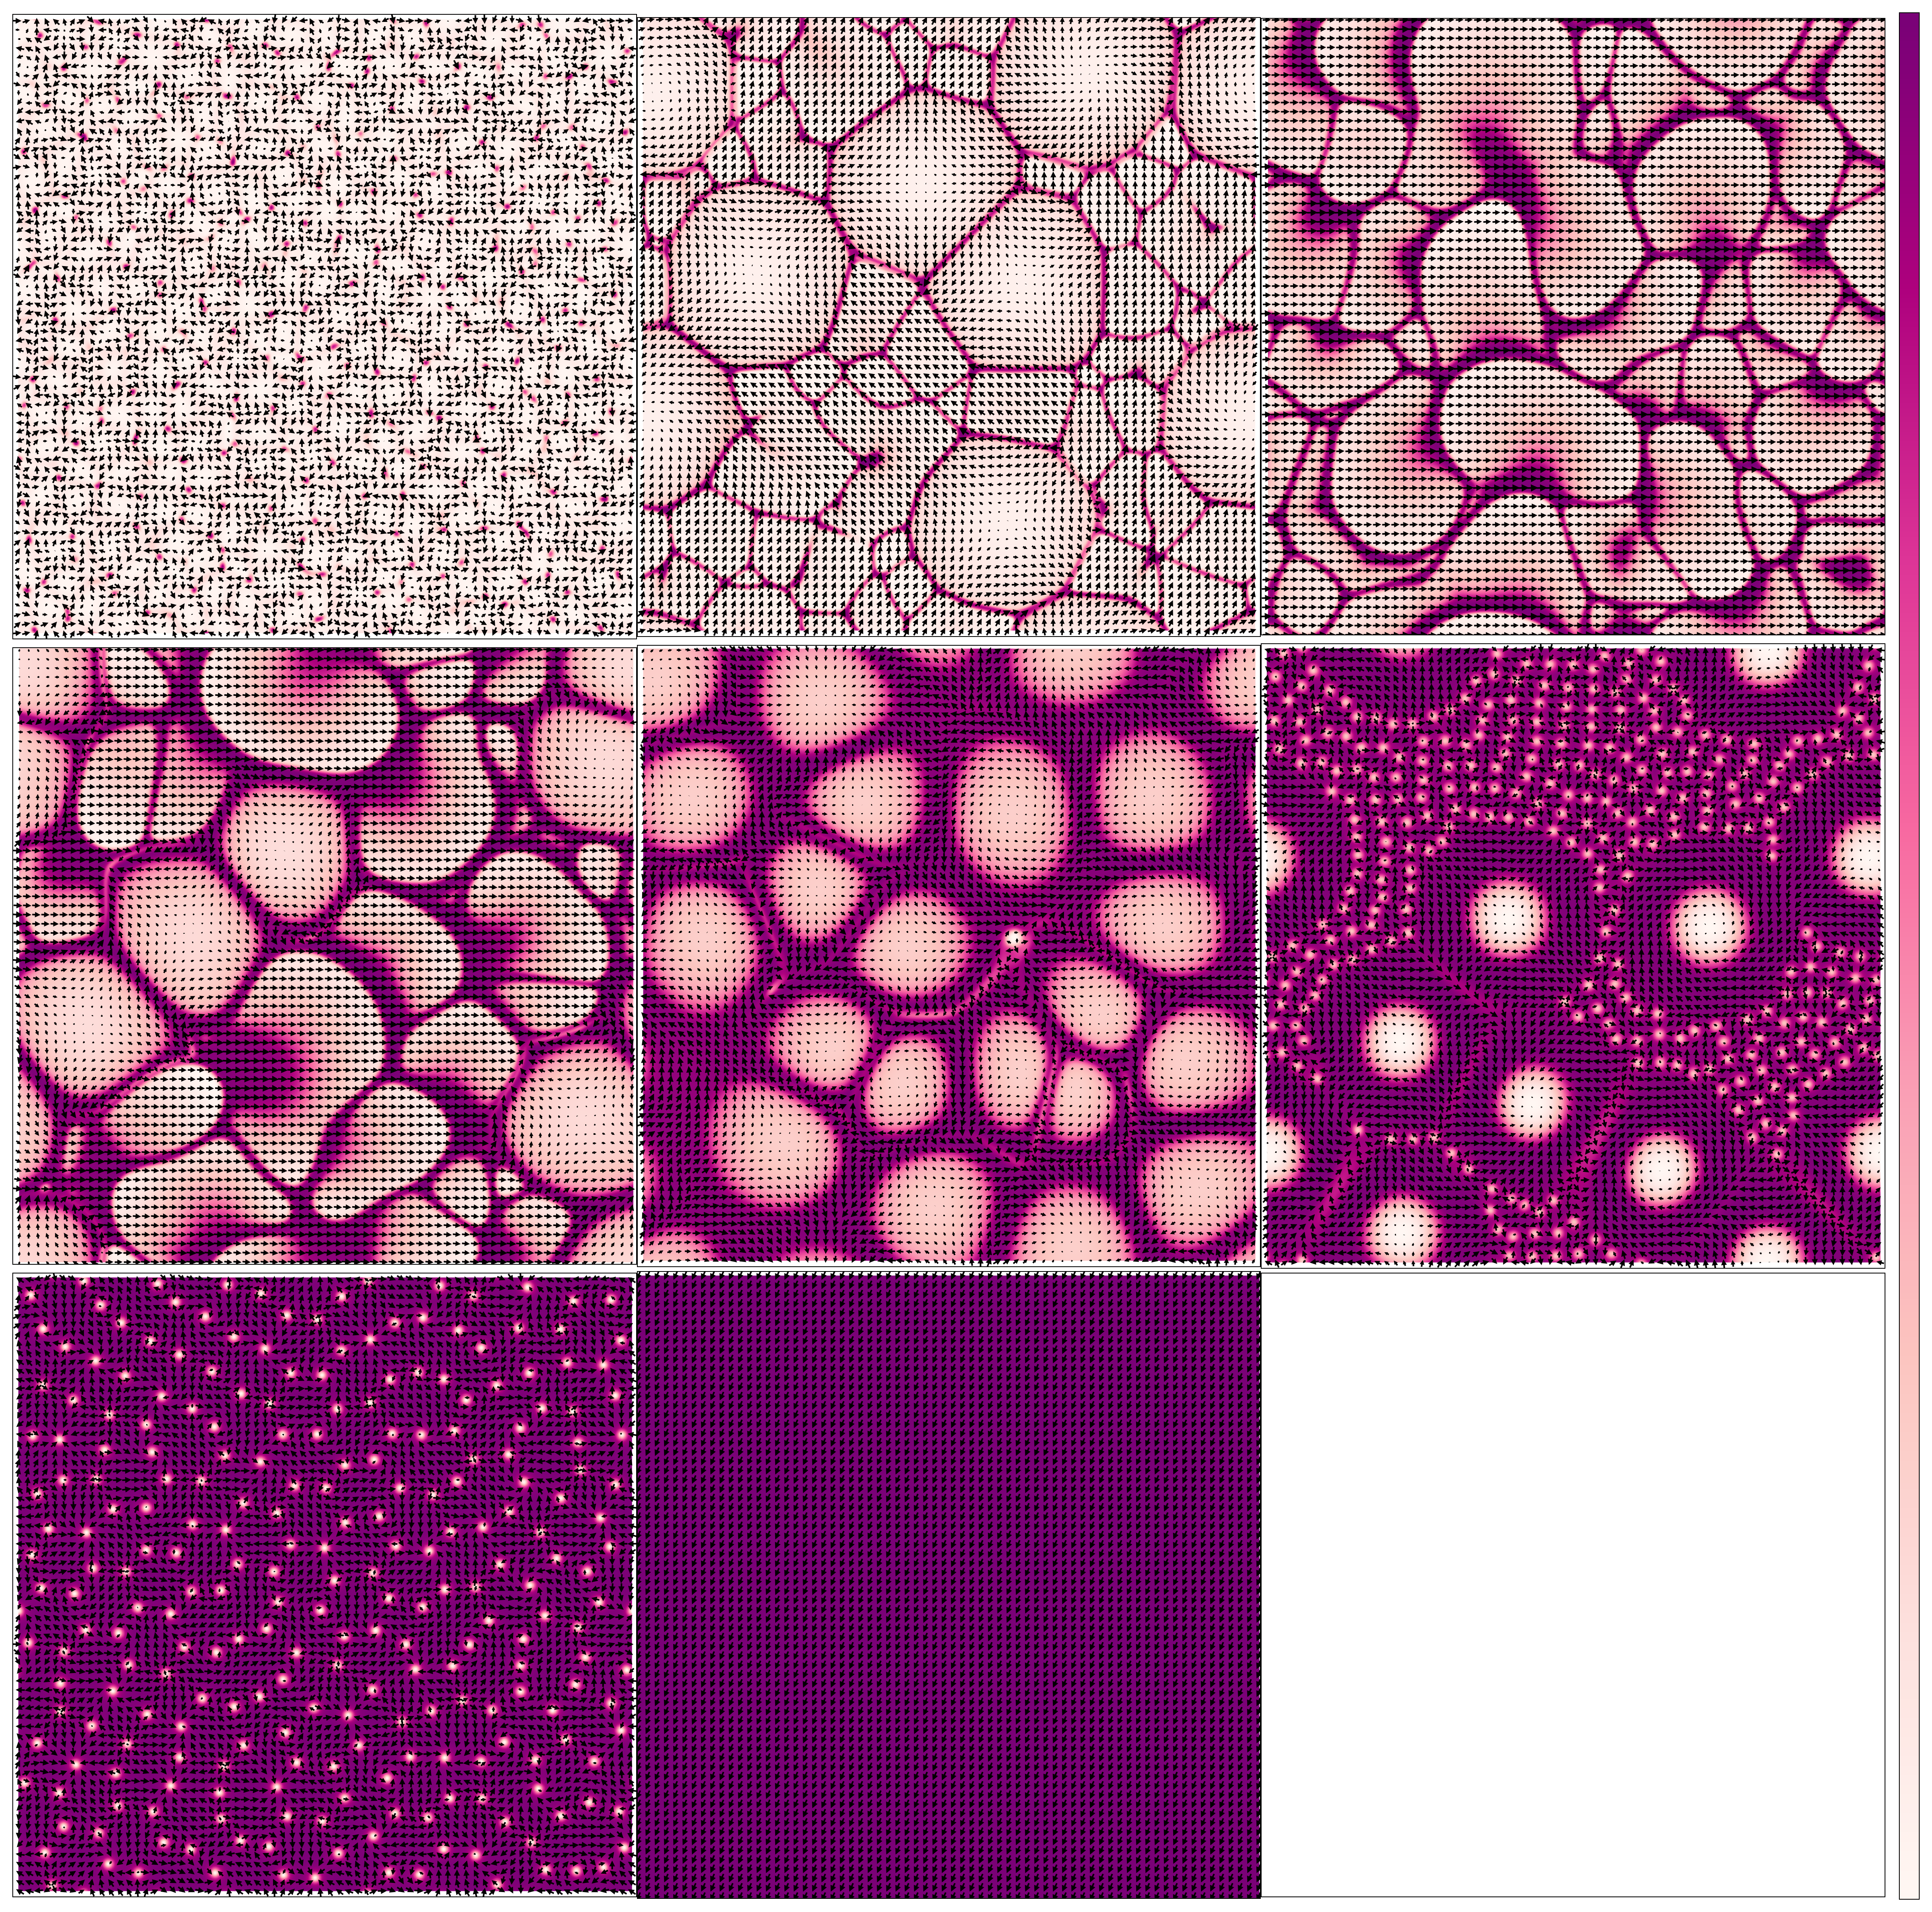
\includegraphics[width=\lx\linewidth]{phases_0.2_0.4_4_v2.png}};

\node at (0.965*\lx*\linewidth,0.02*\linewidth) {$\rho_{min}$};
\node at (0.965*\lx*\linewidth,0.92*\linewidth) {$\rho_{max}$};
\node at (0.965*\lx*\linewidth,0.5*\linewidth) {$\rho$};

\node[inner sep=0pt, anchor=south west] at (0.575*\linewidth, 0.01*\linewidth) {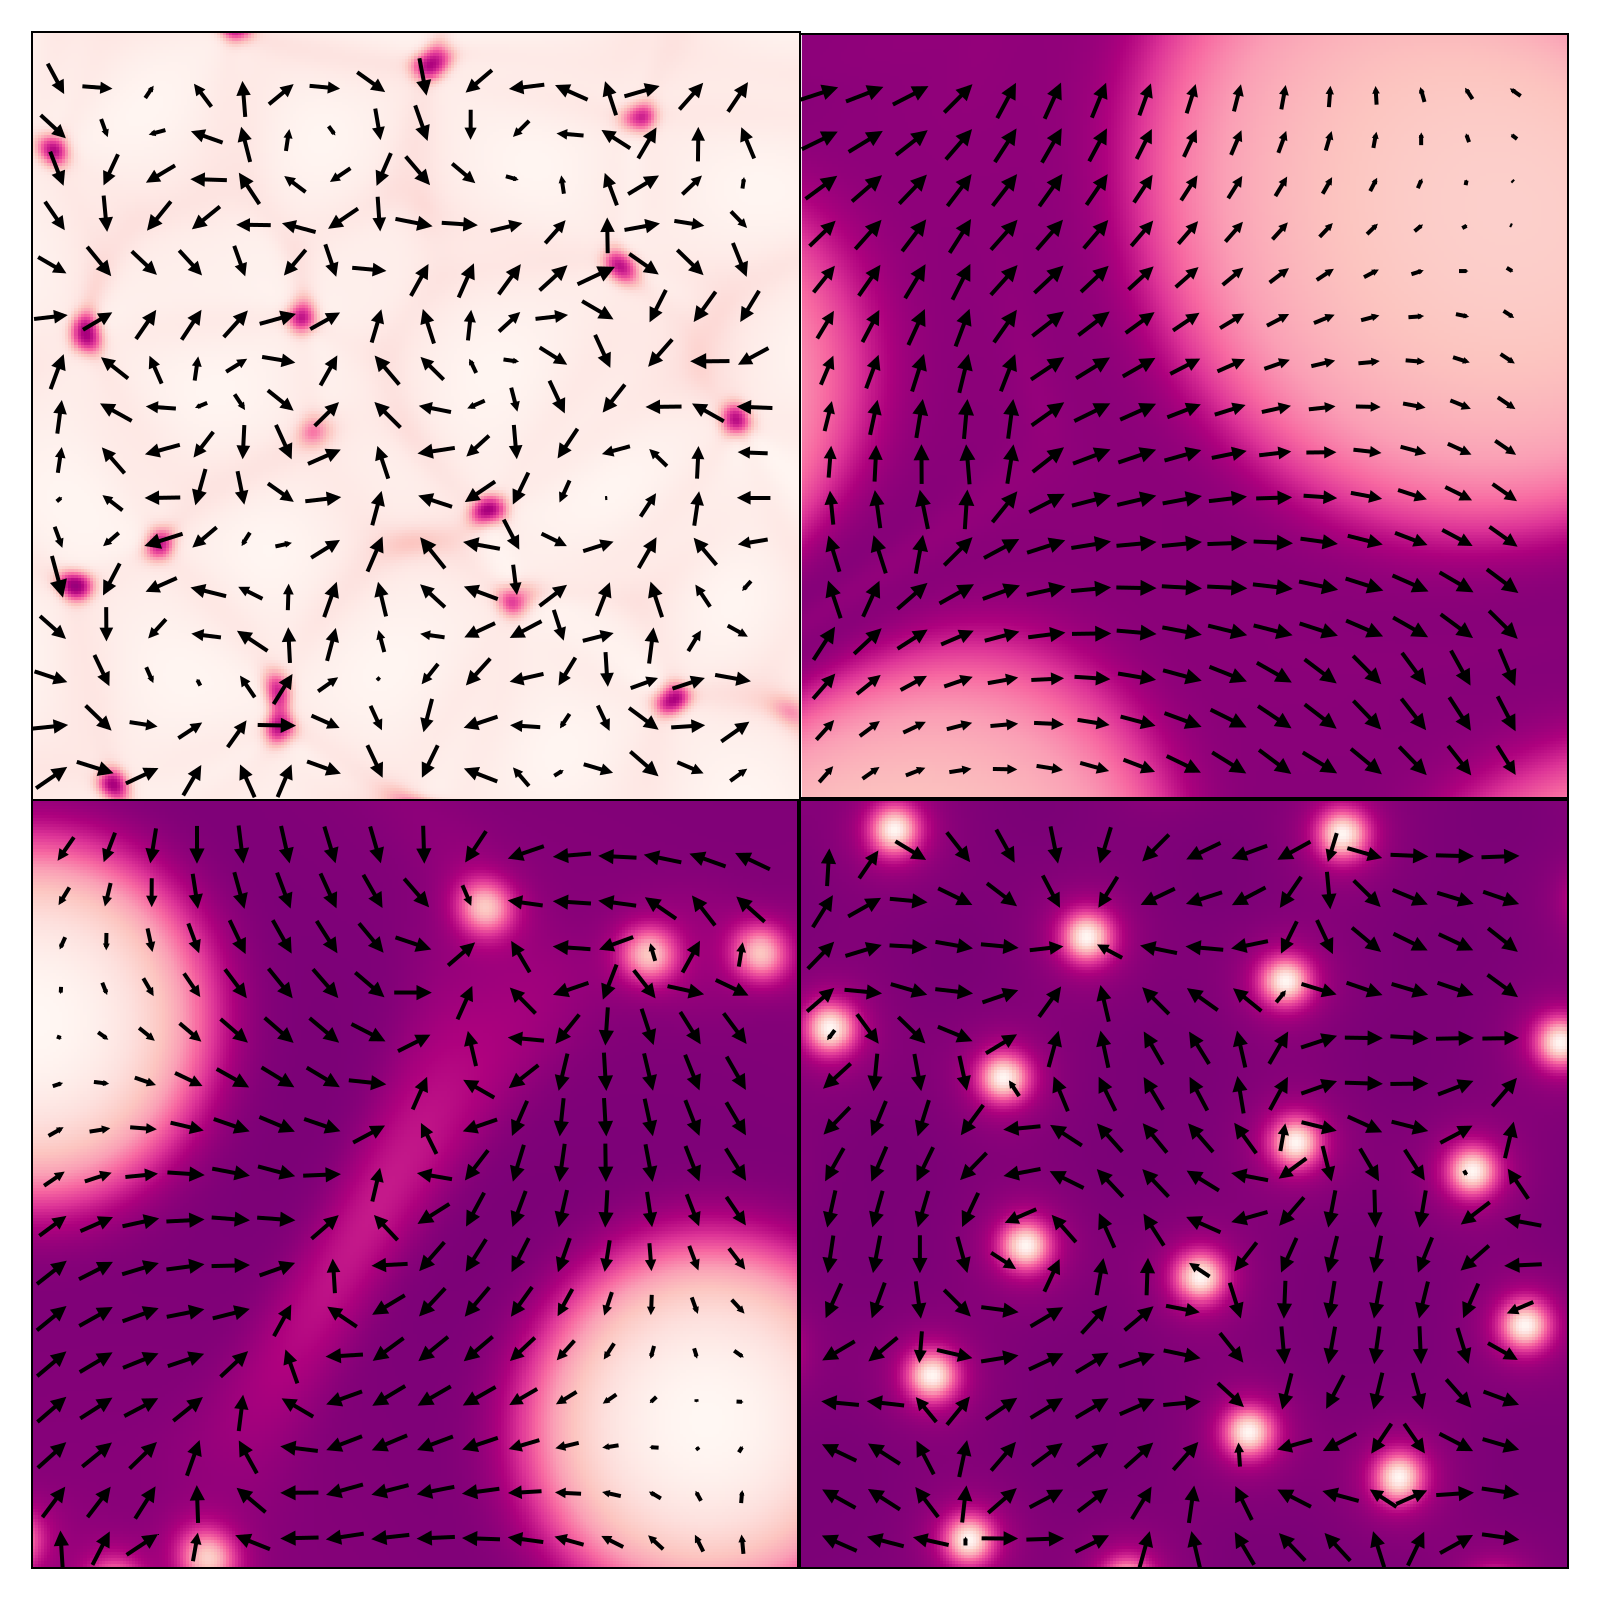
\includegraphics[width=0.3\linewidth]{phases_zoom_0.2_0.4_4_v2.png}};

\node[text = black, rectangle, rounded corners=3pt, fill=white, opacity=0.85, align=center, anchor=south west] at (-0.8*\offx, 0.9*\linewidth) {$\rho_0 = 0.4$};
\node[text = black, rectangle, rounded corners=3pt, fill=white, opacity=0.85, align=center, anchor=south west] at (0.27*\linewidth, 0.9*\linewidth) {$\rho_0 = 0.5$};
\node[text = black, rectangle, rounded corners=3pt, fill=white, opacity=0.85, align=center, anchor=south west] at (0.58*\linewidth, 0.9*\linewidth) {$\rho_0 = 0.6$};
\node[text = black, rectangle, rounded corners=3pt, fill=white, opacity=0.85, align=center, anchor=south west] at (-0.8*\offx, 0.59*\linewidth) {$\rho_0 = 0.65$};
\node[text = black, rectangle, rounded corners=3pt, fill=white, opacity=0.85, align=center, anchor=south west] at (0.27*\linewidth, 0.59*\linewidth) {$\rho_0 = 0.7$};
\node[text = black, rectangle, rounded corners=3pt, fill=white, opacity=0.85, align=center, anchor=south west] at (0.58*\linewidth, 0.59*\linewidth) {$\rho_0 = 0.75$};
\node[text = black, rectangle, rounded corners=3pt, fill=white, opacity=0.85, align=center, anchor=south west] at (-0.8*\offx, 0.28*\linewidth) {$\rho_0 = 0.8$};
\node[text = black, rectangle, rounded corners=3pt, fill=white, opacity=0.85, align=center, anchor=south west] at (0.27*\linewidth, 0.28*\linewidth) {$\rho_0 = 1.2$};

\draw[color=white, ultra thick, anchor=south west] (-0.8*\offx,0.628*\linewidth) rectangle ++ (1.4,1.4);
\draw[color=white, ultra thick, anchor=south west] (0.267*\linewidth,0.32*\linewidth) rectangle ++ (1.4,1.4);
\draw[color=white, ultra thick, anchor=south west] (0.573*\linewidth,0.32*\linewidth) rectangle ++ (1.4,1.4);
\draw[color=white, ultra thick, anchor=south west] (-0.8*\offx,0.01*\linewidth) rectangle ++ (1.4,1.4);

\node[text = black, rectangle, rounded corners=1pt, fill=white, opacity=0.8, anchor=south west] at (-0.8*\offx+1,0.628*\linewidth+1) {\textbf{A}};
\node[text = black, rectangle, rounded corners=1pt, fill=white, opacity=0.8, anchor=south west] at (0.267*\linewidth+1,0.32*\linewidth+1) {\textbf{B}};
\node[text = black, rectangle, rounded corners=1pt, fill=white, opacity=0.8, anchor=south west] at (0.573*\linewidth+1,0.32*\linewidth+1) {\textbf{C}};
\node[text = black, rectangle, rounded corners=1pt, fill=white, opacity=0.8, anchor=south west] at (-0.8*\offx+1,0.01*\linewidth+1) {\textbf{D}};

\node[text = black, rectangle, rounded corners=1pt, fill=white, opacity=0.8, anchor=south west] at (0.585*\linewidth,0.163*\linewidth) {\textbf{A}};
\node[text = black, rectangle, rounded corners=1pt, fill=white, opacity=0.8, anchor=south west] at (0.728*\linewidth,0.163*\linewidth) {\textbf{B}};
\node[text = black, rectangle, rounded corners=1pt, fill=white, opacity=0.8, anchor=south west] at (0.585*\linewidth,0.018*\linewidth) {\textbf{C}};
\node[text = black, rectangle, rounded corners=1pt, fill=white, opacity=0.8, anchor=south west] at (0.728*\linewidth,0.018*\linewidth) {\textbf{D}};

\node[text = black, rectangle, rounded corners=3pt, fill=white, opacity=0.85, anchor=south east] at (0.26*\linewidth, 0.628*\linewidth) {$\begin{aligned} \rho_{max} \approx 0.90\\ \rho_{min} \approx 0.35\end{aligned}$};
\node[text = black, rectangle, rounded corners=3pt, fill=white, opacity=0.85, anchor=south east] at (0.568*\linewidth, 0.628*\linewidth) {$\begin{aligned} \rho_{max} \approx 0.93\\ \rho_{min} \approx 0.41\end{aligned}$};
\node[text = black, rectangle, rounded corners=3pt, fill=white, opacity=0.85, anchor=south east] at (0.875*\linewidth, 0.628*\linewidth) {$\begin{aligned} \rho_{max} \approx 0.86\\ \rho_{min} \approx 0.44\end{aligned}$};
\node[text = black, rectangle, rounded corners=3pt, fill=white, opacity=0.85, anchor=south east] at (0.26*\linewidth, 0.32*\linewidth) {$\begin{aligned} \rho_{max} \approx 0.83\\ \rho_{min} \approx 0.47\end{aligned}$};
\node[text = black, rectangle, rounded corners=3pt, fill=white, opacity=0.85, anchor=south east] at (0.568*\linewidth, 0.32*\linewidth) {$\begin{aligned} \rho_{max} \approx 0.81\\ \rho_{min} \approx 0.48\end{aligned}$};
\node[text = black, rectangle, rounded corners=3pt, fill=white, opacity=0.85, anchor=south east] at (0.875*\linewidth, 0.32*\linewidth) {$\begin{aligned} \rho_{max} \approx 0.78\\ \rho_{min} \approx 0.59\end{aligned}$};
\node[text = black, rectangle, rounded corners=3pt, fill=white, opacity=0.85, anchor=south east] at (0.26*\linewidth, 0.01*\linewidth) {$\begin{aligned} \rho_{max} \approx 0.81\\ \rho_{min} \approx 0.72\end{aligned}$};
\node[text = black, rectangle, rounded corners=3pt, fill=white, opacity=0.85, anchor=south east] at (0.568*\linewidth, 0.01*\linewidth) {$\begin{aligned} \rho_{max} = \rho_0\\ \rho_{min} =\rho_0 \end{aligned}$};

\end{tikzpicture}%
\end{document}
